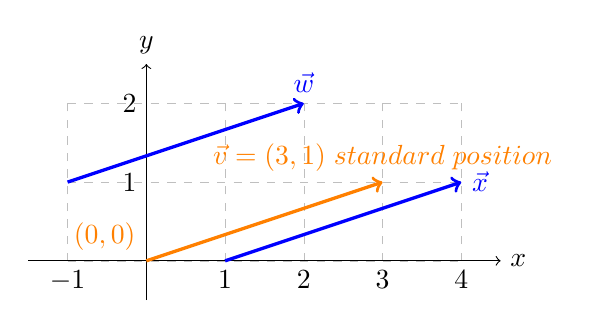
\begin{tikzpicture}
    \draw[step=1,help lines, dashed,lightgray] (-1,0) grid (4,2);
    %draw axis value
    \foreach \x in {-1,1,2,3,4}
        {%
            \draw (\x,0) -- (\x,0) node [below] {$\x$};
        }
    \foreach \y in {1,2}
        {%
            \draw (0,\y) -- (0,\y) node [left] {$\y$};
        }
    %draw lines
    \draw [->] (-1.5,0) -- (4.5,0) node[right]{$x$};
    \draw [->] (0,-0.5) -- (0,2.5) node[above]{$y$};
    \draw [->,blue,very thick] (-1,1) -- (2,2) node[above]{$\vec{w}$};
    \draw [->,orange,very thick] node[above left]{$(0,0)$} (0,0) -- (3,1) node[above]{$\vec{v}=(3,1)\hspace{0.1cm} standard\hspace{0.1cm} position$};
    \draw [->,blue,very thick] (1,0) -- (4,1) node[right]{$\vec{x}$};
\end{tikzpicture}
\captionof{figure}{{\footnotesize standard position vector vs non-standard position vector}}
\label{fig:vector-and-vector-operation-d1}
